\documentclass[10pt,xcolor=dvipsnames]{beamer}
\usepackage[french]{babel}
\usepackage[utf8]{inputenc}
\usepackage[T1]{fontenc}
\usepackage{caption}
\usepackage{MnSymbol,wasysym}
\usepackage{amsmath}
\usepackage{cancel}
\usepackage[draft]{pdfcomment}
\newcommand{\pdfnote}[1]{\marginnote{\pdfcomment[icon=note]{#1}}}
\usepackage{appendixnumberbeamer}
\usepackage{comment}

\usepackage{pifont}% http://ctan.org/pkg/pifont
\newcommand{\cmark}{\textbf{\textcolor{darkspringgreen}{\ding{51}}}}%
\newcommand{\xmark}{\textbf{\textcolor{red}{\ding{55}}}}%


\renewcommand{\thefootnote}{\fnsymbol{footnote}}



\newcommand*\Let[2]{\State #1 $\gets$ #2}
\usepackage{algorithm}
\usepackage[noend]{algpseudocode}
\usepackage{tcolorbox}

\newtcolorbox{mybox}[3][]
{
  colframe = #2!25,
  colback  = #2!10,
  coltitle = #2!20!black,  
  title    = {#3},
  #1,
}

\usetheme[progressbar=frametitle,numbering=fraction]{metropolis}
%LS:
\setbeamercolor{background canvas}{bg=white}  
\usepackage{appendixnumberbeamer}

\usepackage{booktabs}
\usepackage[scale=2]{ccicons}
\usepackage{tikz}
\usetikzlibrary{calc}
\usepackage{color}
\usepackage{mathtools}

\usetikzlibrary{shapes,snakes}
%% Color Definition
\definecolor{darkspringgreen}{rgb}{0.09, 0.45, 0.27}
\definecolor{push}{HTML}{00AF37}
\definecolor{pull}{HTML}{3319BC}

\newcommand{\push}[1]{\textcolor{push}{push(#1)}}
\newcommand{\pull}[1]{\textcolor{pull}{pop(#1)}}
\newcommand{\pop}{\textcolor{pull}{pop()}}

\newcommand{\defin}[1]{\textcolor{darkspringgreen}{#1}}
\setbeamertemplate{frame footer}{Rohan Fossé}

\setbeamercolor{footline}{fg=gray}

\def\checkmark{\tikz\fill[scale=0.4,color=darkspringgreen](0,.35) -- (.25,0) -- (1,.7) -- (.25,.15) -- cycle;}
\usepackage{pgfplots}
\usepgfplotslibrary{dateplot}

\usepackage{eso-pic}
\usepackage{xspace}
\long\def\/*#1*/{}

\title{
Algorithmique et structure de données
}
\subtitle{Structures de données}

\date{\centering 11 Octobre 2021}
\author{\centering \bf Rohan Fossé}


\begin{document}

\maketitle



\begin{frame}{Algorithmes et structures de données}
    La plupart des bons algorithmes fonctionnent grâce à une méthode astucieuse pour organiser les données. Nous allons étudier cinq classes de structures de données :
    \begin{itemize}
        \item les \alert{tableaux};
        \item les \alert{piles};
        \item les \alert{listes};
        \item les \alert{files};
        \item les \alert{arbres}.
    \end{itemize}
\end{frame}

\section{Structure séquentielles: les tableaux}

\begin{frame}{Structure de donnée séquentielle : tableau}

En anglais : array, vector.

\begin{exampleblock}{Définition}
    Un \textbf{tableau} est une structure de donnée $T$ qui permet de stocker un certain nombre d'éléments $T[i]$ repérés par un index $i$. Les tableaux vérifient généralement les propriétés suivantes :
    \begin{itemize}
        \item tous les éléments ont le même type de base;
        \item le nombre d'éléments stockés est fixé;
        \item l'accès et la modification de l'élément numéro $i$ est en temps constant $\mathcal{O}(1)$, indépendant de $i$ et du nombre d'éléments dans le tableau.
    \end{itemize}
\end{exampleblock}
    
\end{frame}

\begin{frame}{Opérations de base}
    Hypothèses :
    \begin{itemize}
        \item tableau de taille $capacite$ alloué;
        \item éléments $ 0 \leq i \leq taille \leq capacite$ initialisés
    \end{itemize}
    
    \begin{alertblock}{A retenir}
    \begin{itemize}[<+->]
        \item accès au premier élément : $\mathcal{O}(1)$;
        \item accès à l'élément numéro $i$ : $\mathcal{O}(1)$;
        \item accès au dernier élément : $\mathcal{O}(1)$;
        \item insertion/suppression d'un élément au début : $\mathcal{O}(taille)$;
        \item insert./suppr. d'un elt en position $i$ : $\mathcal{O}(taille - i)$
        \item insert./suppr. d'un elt à la fin : $\mathcal{O}(1)$;
    \end{itemize}
    \end{alertblock}
\end{frame}


\section{Les piles}

\begin{frame}{Définition}
    \begin{exampleblock}{définition}
Une \defin{pile} est une liste linéaire d'objets où les consultations, les insertions et les suppressions se font du même côté. On dit que c'est le \defin{dernier arrivé, premier servi}.
\end{exampleblock}

\only<2>{
\begin{figure}
    \centering
    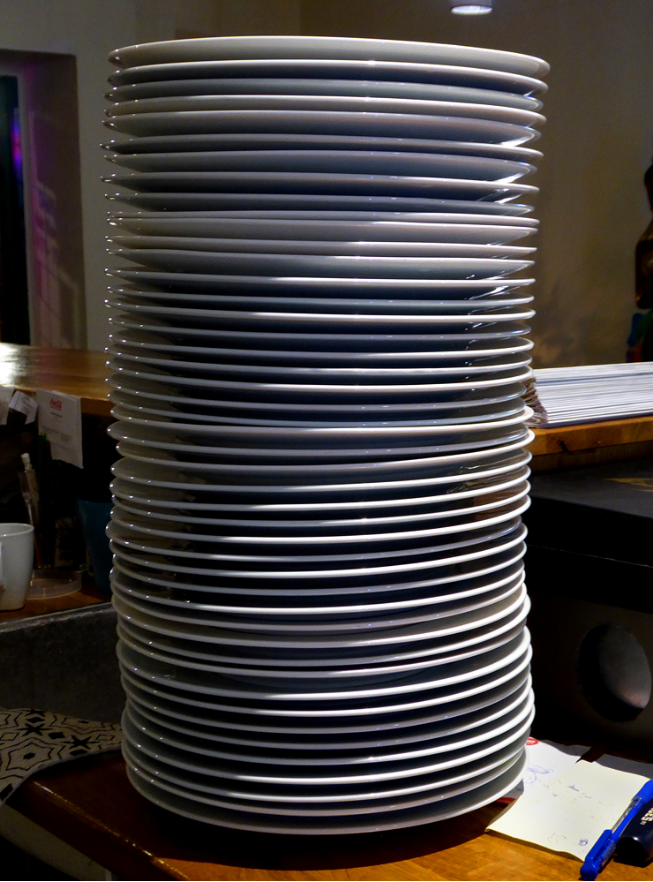
\includegraphics[scale=0.18]{figures/CM2/assiette.png}
    \label{fig:my_label}
\end{figure}
}

\only<3>{
\begin{figure}
    \centering
    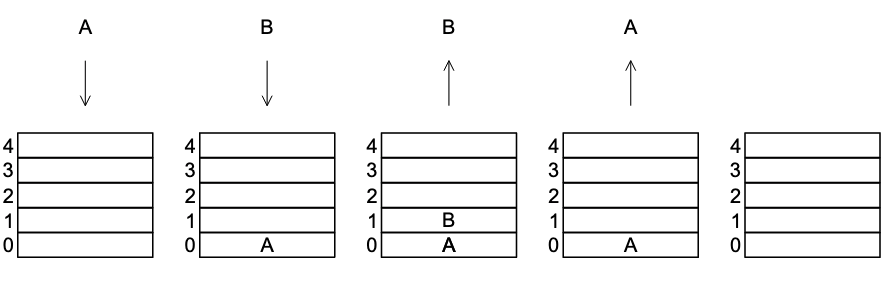
\includegraphics[scale=0.3]{figures/CM2/pile-formel.png}
    \label{fig:my_label}
\end{figure}
}

\only<4>{

\begin{alertblock}{Vocabulaire}
Le vocabulaire est basé sur une représentation verticale et est essentiellement en anglais, entre parenthèses ici:
\begin{itemize}
    \item Dernier arrivé, premier servi ( \textit{Last-in-first-out} ou \textit{LIFO} );
    \item pile ( \textit{stack} );
    \item empiler ( \textit{push} );
    \item dépiler ( \textit{pop} );
    \item sommet ( \textit{top} );
    \item pile vide ( \textit{empty} )
\end{itemize}
\end{alertblock}

}

\end{frame}

\begin{frame}{Opérations sur les piles}
    Les opérations sur la pile peuvent impliquer l'initialisation de la pile, son utilisation et sa dé-initialisation. En dehors de ces opérations de base, une pile est utilisée pour les deux opérations principales suivantes
\begin{itemize}
    \item \textit{push()} - Pousser (stocker) un élément sur la pile;
    \item \textit{pop()} - Retirer (accéder à) un élément de la pile.
\end{itemize}
   
Pour utiliser efficacement une pile, nous devons également vérifier l'état de la pile, les fonctionnalités suivantes sont ajoutées aux piles : 

\begin{itemize}
    \item peek() - obtient l'élément de données supérieur de la pile, sans le supprimer;
    \item isFull() - Vérifie si la pile est pleine;
    \item isEmpty() - vérifie si la pile est vide.
\end{itemize}
    Le pointeur \alert{top} fournit la valeur supérieure de la pile sans la supprimer réellement.
\end{frame}

\begin{frame}{Première opération : Peek}
    \begin{exampleblock}{Définition}
    La fonction $peek()$ permet d'obtenir l'élément de données supérieur de la pile, sans le supprimer.
    \end{exampleblock}

    \begin{tcolorbox}

  \begin{algorithmic}[1]
    \Function{$peek$}{}
       \State\text{\textbf{return}} $stack[top]$
    \EndFunction
  \end{algorithmic}
 \end{tcolorbox}
\end{frame}

\begin{frame}{Deuxième opération : isFull}
    \begin{exampleblock}{Définition}
    La fonction $isFull()$ permet de vérifier si la pile est pleine.
    \end{exampleblock}

        \begin{tcolorbox}
  \begin{algorithmic}[1]
    \Function{$isFull$}{}
       \If{$\text{top == MAXSIZE}$}
            \State\text{\textbf{return}} $true$
       \Else
            \State\text{\textbf{return}} $false$
       \EndIf
    \EndFunction
  \end{algorithmic}
 \end{tcolorbox}
\end{frame}

\begin{frame}{Troisième opération : isEmpty}
    \begin{exampleblock}{Définition}
    La fonction $isEmpty()$ permet de vérifier si la pile est vide.
    \end{exampleblock}
    
            \begin{tcolorbox}
  \begin{algorithmic}[1]
    \Function{$isEmpty$}{}
       \If{$\text{top < 1}$}
            \State\text{\textbf{return}} $true$
       \Else
            \State\text{\textbf{return}} $false$
       \EndIf
    \EndFunction
  \end{algorithmic}
 \end{tcolorbox}
\end{frame}

\begin{frame}{Opération push}
    Le processus consistant à placer un nouvel élément de données sur la pile est connu sous le nom d'opération \alert{push}. L'opération \alert{push} comporte une série d'étapes:

\only<1>{
   \begin{enumerate}
       \item on vérifie si la pile est pleine;
       \item si la pile est pleine, on retourne une erreur;
       \item si la pile n'est pas pleine, on incrémente \textit{top} jusqu'au prochain espace vide;
       \item  Ajoute un élément à l'emplacement de la pile où $top$ pointe.
   \end{enumerate}
}

\only<2>{

\begin{figure}
    \centering
    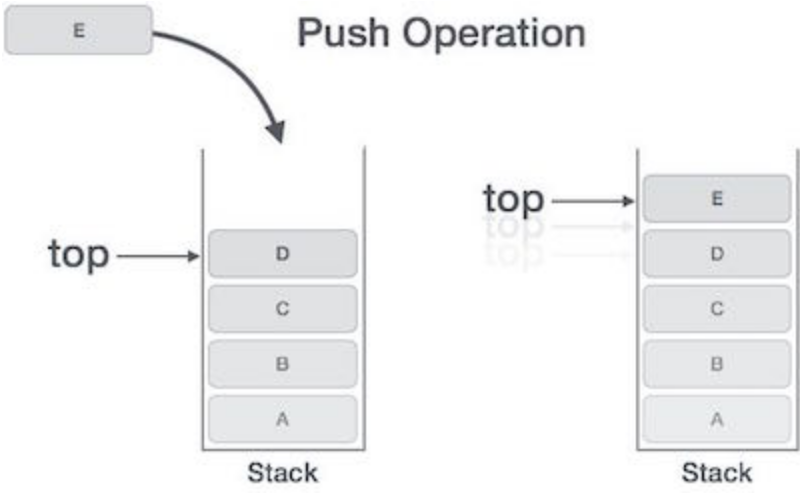
\includegraphics[scale=0.25]{figures/CM2/push.png}
    \label{fig:my_label}
\end{figure}

}

\only<3>{

\begin{tcolorbox}
  \begin{algorithmic}[1]
    \Function{$push$}{$data$}
       \If{$\text{stack.isfull()}$}
            \State\text{\textbf{return}} $null$
       \EndIf
            \Let{$top$}{$top + 1$}
            \Let{$stack[top]$}{$data$}
    \EndFunction
  \end{algorithmic}
\end{tcolorbox}
}
\end{frame}

\begin{frame}{Opération pop}

    \only<1-2>{
Accéder au contenu tout en le retirant de la pile est connu sous le nom d'opération \alert{pop}.
    La fonction change suivant l'implémentation de la pile:
    \begin{itemize}
        \item Si elle a été implémenté avec un \alert{tableau},  l'élément n'est pas réellement supprimé, mais le sommet est décrémenté à une position inférieure dans la pile pour pointer vers la valeur suivante;
        \item si elle a été implementé avec une \alert{liste chaînée}, l'opération $pop()$ supprime réellement l'élément de données et désalloue l'espace mémoire.
    \end{itemize}
    }
    \only<3>{
L'opération \alert{pop} comporte une série d'étapes:
    \begin{enumerate}
        \item On vérifie si la pile est vide;
        \item si elle est effectivement vide, on retourne une erreur;
        \item sinon, on accède à l'élément $data$ où $top$ pointe;
        \item on décroit la valeur de $top$ de 1;
        \item on retourne $data$
    \end{enumerate}
    }
    
    \only<4>{
    
        Le processus consistant à récupérer un élément de données sur la pile est connu sous le nom d'opération \alert{pop}. L'opération \alert{pop} comporte une série d'étapes:
    \begin{figure}
        \centering
        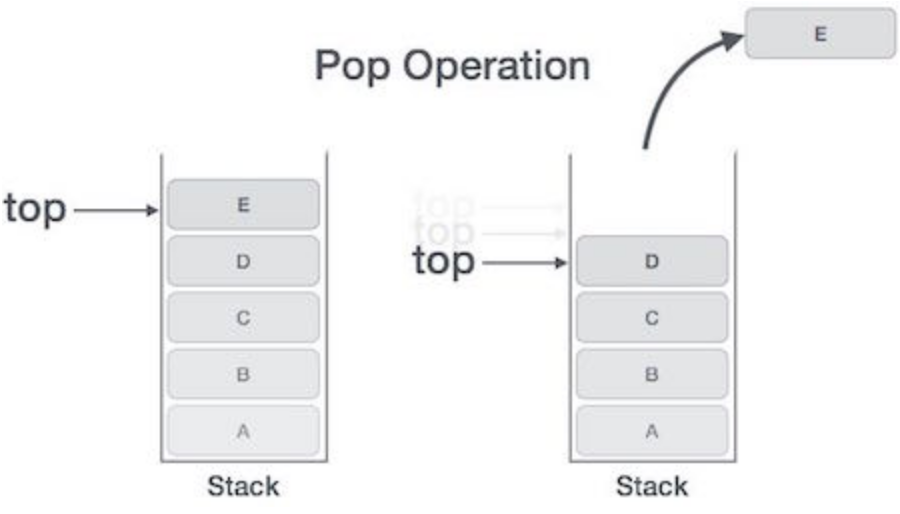
\includegraphics[scale=0.28]{figures/CM2/pop.png}
        \label{fig:my_label}
    \end{figure}
    }

    \only<5>{
            Le processus consistant à récupérer un élément de données sur la pile est connu sous le nom d'opération \alert{pop}. L'opération \alert{pop} comporte une série d'étapes:
        \begin{tcolorbox}
  \begin{algorithmic}[1]
    \Function{$pop$}{}
       \If{$\text{stack.isEmpty()}$}
            \State\text{\textbf{return}} $null$
       \EndIf
            \Let{$data$}{$stack[top]$}
            \Let{$top$}{$top - 1$}
            \State\text{\textbf{return}} $data$
    \EndFunction
  \end{algorithmic}
\end{tcolorbox}
    }
\end{frame}

\begin{frame}{Petit exercice sur les piles}
    On suppose que une séquence d'opérations \alert{$push$} et \alert{$pop$} sont faites sur une pile $P$. On suppose que les opérations \alert{$push$} empilent les entiers $\{0,1,2,3,4,5,6,7,8,9\}$ dans l'ordre croissant et que toute valeur dépilée avec \alert{$pop$} est affichée. On souhaite afficher toutes les valeurs.
    \only<1-2>{
        \begin{exampleblock}{Exemple}
        Considérons la séquence d'opérations suivante :
        \begin{equation*}
            \push{1} \rightarrow \push{2} \rightarrow \push{3} \rightarrow \pop \rightarrow \pop \rightarrow \push{2}
        \end{equation*}
        Cette séquence va afficher :
        \only<2>{
        \begin{equation*}
            3 \quad 2
        \end{equation*}
        }
        
        \end{exampleblock}
    }
    
\only<3>{
\begin{alertblock}{Exercice}
    Dire quelle séquence de valeurs affichées n'est pas possible. Si elle l'est, donner la séquence d'opérations permettant de l'obtenir.
\begin{enumerate}
\item 4 3 2 1 0 9 8 7 6 5
\item 4 6 8 7 5 3 2 9 0 1 
\item 2 5 6 7 4 8 9 3 1 0
\item 4 3 2 1 0 5 6 7 8 9
\end{enumerate}
\end{alertblock}
}
\end{frame}

\begin{frame}{Solution de l'exercice}
    \begin{enumerate}
\alert{\item 4 3 2 1 0 9 8 7 6 5} \cmark
\item 4 6 8 7 5 3 2 9 0 1 
\item 2 5 6 7 4 8 9 3 1 0
\item 4 3 2 1 0 5 6 7 8 9
\end{enumerate}

\begin{alertblock}{Solution}
  \begin{equation*}
            \push{0-4} \rightarrow \pull{4-0} \rightarrow \push{5-9} \rightarrow \pull{9-5}
\end{equation*}
\end{alertblock}

\end{frame}

\begin{frame}{Solution de l'exercice}


    \begin{enumerate}
\item 4 3 2 1 0 9 8 7 6 5
\alert{\item 4 6 8 7 5 3 2 9 0 1} \xmark
\item 2 5 6 7 4 8 9 3 1 0
\item 4 3 2 1 0 5 6 7 8 9
\end{enumerate}

\begin{alertblock}{Solution}
  \begin{equation*}
            \push{0-4} \rightarrow \pull{4} \rightarrow \push{5-6} \rightarrow \pull{6} \rightarrow \push{7-8} \rightarrow \pull{8}
\end{equation*}
\begin{equation*}
                \rightarrow \pull{7} \rightarrow \pull{5} \rightarrow \pull{3} \rightarrow \pull{2} \rightarrow \push{9} \rightarrow \pull{9} \rightarrow \xmark
\end{equation*}
\end{alertblock}
\end{frame}


\begin{frame}{Solution de l'exercice}
    \begin{enumerate}
\item 4 3 2 1 0 9 8 7 6 5
\item 4 6 8 7 5 3 2 9 0 1 
\alert{\item 2 5 6 7 4 8 9 3 1 0} \cmark
\item 4 3 2 1 0 5 6 7 8 9
\end{enumerate}

\begin{alertblock}{Solution}
  \begin{equation*}
            \push{0-2} \rightarrow \pull{2} \rightarrow \push{3-5} \rightarrow \pull{5} \rightarrow \push{6}
\end{equation*}
\begin{equation*}
    \rightarrow \pull{6} \rightarrow \push{7} \rightarrow \pull{7} \rightarrow \pull{4} \rightarrow \push{8} \rightarrow \pull{9}
\end{equation*}
\begin{equation*}
     \rightarrow \push{9} \rightarrow \pull{9} \rightarrow \pull{3} \rightarrow \pull{1} \rightarrow \pull{0}    
\end{equation*}
\end{alertblock}
\end{frame}


\begin{frame}{Solution de l'exercice}
    \begin{enumerate}
\item 4 3 2 1 0 9 8 7 6 5
\item 4 6 8 7 5 3 2 9 0 1 
\item 2 5 6 7 4 8 9 3 1 0
\alert{\item 4 3 2 1 0 5 6 7 8 9} \cmark 
\end{enumerate}

\begin{alertblock}{Solution}
  \begin{equation*}
            \push{0-4} \rightarrow \pull{4-0} \rightarrow \push{5} \rightarrow \pull{5} \rightarrow \push{6} \rightarrow
\end{equation*}
\begin{equation*}
 \pull{6} \rightarrow \push{7} \rightarrow \pull{7} \rightarrow \push{8} \rightarrow \pull{8} \rightarrow \push{9} \rightarrow \pull{9}
\end{equation*}
\end{alertblock}

\end{frame}


\begin{frame}{Exemples d'utilisation des piles}

\begin{itemize}
    \item  Les algorithmes récursifs utilisent une pile d'appel;
    \item  Dans un navigateur web, une pile sert à mémoriser les pages Web visitées;
    \item     La fonction « Annuler la frappe » (en anglais Undo) d'un traitement de texte mémorise les modifications apportées au texte dans une pile;
    \item Par exemple, on peut inverser un tableau ou une chaîne de caractères en utilisant une pile;
    \item L'évaluation des expressions mathématiques en notation \textit{post-fixée} (ou polonaise inverse) utilise une pile. \alert{Qu'est-ce-que c'est ?}
    
\end{itemize}
\end{frame}

\begin{frame}{Les différentes notations}
    La manière d'écrire une expression arithmétique est connue sous le nom de \alert{notation}. Une expression arithmétique peut être écrite dans trois notations différentes mais équivalentes, c'est-à-dire sans changer la sortie d'une expression. Ces notations sont les suivantes:

\begin{itemize}
    \item Notation infixe;
    \item Notation préfixe (polonaise);
    \item Notation postfixe (polonaise inversée).
\end{itemize}


\end{frame}

\begin{frame}{Notation infixe}
    Nous écrivons naturellement les expressions en notation \alert{infixe} (par exemple a - b + c), où les opérateurs sont utilisés entre les opérandes.\\
    Il est facile pour nous, humains, de lire, d'écrire et de parler en notation infixe, mais ça n'est pas aussi simple pour un ordinateur.\\
    Un algorithme pour traiter la notation infixe pourrait être difficile et coûteux en termes de temps et d'espace.
\end{frame}


\begin{frame}{Notation préfixe}
    Dans la notation préfixe, l'opérateur précède les deux opérandes.
    
    \begin{table}[]
\begin{tabular}{cc}
\textbf{infixe} & \textbf{prefixe} \\
2+3             & + 2 3            \\
p-q             & - p q            \\
a + b * c       & + a * b c       
\end{tabular}
\end{table}
\end{frame}

\begin{frame}{Notation postfixe (notation polonaise inversée )}
     Dans la notation préfixe, l'opérateur est écrit après les deux opérandes.
     
     \begin{table}[]
\begin{tabular}{ccc}
\textbf{infixe} & \textbf{prefixe} & \textbf{postfixe} \\
2+3             & + 2 3            & 2 3 +             \\
p-q             & - p q            & p q -             \\
a + b * c       & + a * b c        & a b c * +        
\end{tabular}
\end{table}

\only<2>{\alert{A quoi ça sert ?}}
\end{frame}

\begin{frame}{Conversion d'une expression infixe à postfixe}
    Supposons que l'on ait l'expression :
    \begin{equation*}
        a * b + c * d - e
    \end{equation*}
    \only<2>{De façon équivalente, on peut l'écrire de la façon suivante :
    \begin{equation*}
        [(a * b) + (c * d) ] - e
    \end{equation*}
    }
    \only<3->{
    On peut maintenant changer l'expression en expression posfixe :
    }
    \begin{equation*}
        \only<3>{
            [(a b *) + (c d *) ] - e
        }
        \only<4>{
            [(a b *) (c d *) + ] - e
        }
        \only<5->{
            [(a b *) (c d *) + ] e -
        }
    \end{equation*}
    \only<6>{
    On obtient donc à la fin :
    \begin{equation*}
        a b * c d * + e -
    \end{equation*}
    }
\end{frame}



\begin{frame}{Évaluation d'une expression postfixe}
    Reprenons notre expression postfixe :
    \begin{equation*}
        a b * c d * + e -
    \end{equation*}
    Supposons que l'on a :
    \begin{equation*}
        a=2, b=3, c=5, d=4, e=9
    \end{equation*}
    On obtient donc :
    \begin{equation*}
        \only<1>{
        \alert{2 3 *} 5 4 * + 9 -
        }
        \only<2>{
        6 \alert{5 4 *} + 9 -
        }
        \only<3>{
        \alert{6 20 +} 9 -
        }
        \only<4>{
        \alert{26 9 -}
        }
        \only<5>{
        17
        }
    \end{equation*}
\end{frame}

\begin{frame}{Quel est l'algorithme ?}
\begin{exampleblock}{Rappel}
\begin{itemize}
    \item En mathématiques, Un opérateur binaire est un opérateur qui opère sur deux opérandes (comme l'addition;
    \item les opérateurs unaires agissent sur un seul opérande pour produire une nouvelle valeur.
\end{itemize}
\end{exampleblock}
    On utilise pour cela une \alert{pile} initialement vide. On lit successivement chacun des termes de l'expression et on applique l'une des trois règles suivantes selon la nature de ce terme:

\begin{enumerate}
    \item C'est un opérande, on l'empile.
    \item C'est un opérateur binaire $\triangle$ , on dépile la valeur y au sommet de la pile puis la valeur x, puis on empile le résultat de l'opération x $\triangle$ y
    \item C'est un opérateur unaire $\bigstar$ , on dépile la valeur x au sommet de la pile, puis on empile le résultat de l'opération $\bigstar$ x;
\end{enumerate}
\end{frame}

\begin{frame}{Prenons un exemple}
\begin{exampleblock}{Rappel des règles}
        \begin{enumerate}
    \item C'est un opérande, on l'empile.
    \item C'est un opérateur binaire $\triangle$ , on dépile la valeur y au sommet de la pile puis la valeur x, puis on empile le résultat de l'opération x $\triangle$ y
    \item C'est un opérateur unaire $\bigstar$ , on dépile la valeur x au sommet de la pile, puis on empile le résultat de l'opération $\bigstar$ x;
\end{enumerate}
\end{exampleblock}
\only<2>{
Considérons l'expression postfixe suivante :
}
\begin{equation*}
    1.2 \quad 5 * 3 * 3 \quad 1 - 2 * 3 * +
\end{equation*}
\only<3>{
\begin{table}
\centering
\begin{tabular}{|l|l|l|l|l|l|l|l|l|l|l|l|l|l|l|} 
\hline
                             &                      &                    &                    &                    &                    &                    & 1                  &                    & 2                  &                    & 3                  &                    &                      &                               \\ 
\hline
                             &                      & 5                  &                    & 3                  &                    & 3                  & 3                  & 2                  & 2                  & 4                  & 4                  & 12                 &                      &                               \\ 
\hline
                             & 1.2                  & 1.2                & 6                  & 6                  & 18                 & 18                 & 18                 & 18                 & 18                 & 18                 & 18                 & 18                 & 30                   &                               \\ 
\hline
\textcolor{red}{$\emptyset$} & \textcolor{red}{1.2} & \textcolor{red}{5} & \textcolor{red}{*} & \textcolor{red}{3} & \textcolor{red}{*} & \textcolor{red}{3} & \textcolor{red}{1} & \textcolor{red}{-} & \textcolor{red}{2} & \textcolor{red}{*} & \textcolor{red}{3} & \textcolor{red}{*} & \textcolor{red}{$+$} & \textcolor{red}{$\emptyset$}  \\
\hline
\end{tabular}
\end{table}

}
\end{frame}

\begin{frame}{Quel est l'algorithme ?}
        \begin{tcolorbox}
  \begin{algorithmic}[1]
    \Function{$evaluationpostfix$}{$E$}
      \Let{$stack$}{$createStack()$}
      \For{$\text{chaque caractère ch dans l'expression postixe E}$}
          \If{$\text{ ch est un opérateur} \bigstar $}
            \Let{$a$}{$stack.pop()$}
            \Let{$b$}{$stack.pop()$}
            \Let{$res$}{$b \bigstar a$}
          \EndIf
          \If{$\text{ch est un opérateur} \triangle$}
            \Let{$a$}{$stack.pop()$}
            \Let{$res$}{$\triangle a$}
          \Else
            \State \text{$stack.push(ch)$}
          \EndIf
      \EndFor
      \State\text{\textbf{return}} $top$
    \EndFunction
  \end{algorithmic}
\end{tcolorbox}
\end{frame}

\section{Les listes}

\begin{frame}{Liste chaînée : définition}
    
    \begin{exampleblock}{Définition}
        Une \defin{liste chaînée} désigne en informatique une structure de données représentant une collection ordonnée et de taille arbitraire d'éléments de même type.
    \end{exampleblock}
    
    L'accès aux éléments d'une liste se fait de manière séquentielle : chaque élément permet l'accès au suivant (contrairement au cas du tableau dans lequel l'accès se fait de manière absolue, par adressage direct de chaque cellule du dit tableau).
\end{frame}

\begin{frame}{Le principe}
    Le principe de la liste chaînée est que chaque élément possède, en plus de la donnée, des \alert{pointeurs} vers les éléments qui lui sont logiquement adjacents dans la liste.
    
    \begin{figure}
    \centering
    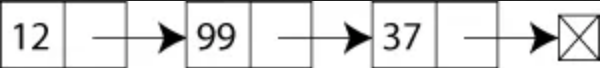
\includegraphics[scale= 0.4]{figures/CM2/liste-chaine.png}
    \label{fig:my_label}
\end{figure}

De ce fait, l'usage d'une liste est préconisé pour des raisons de rapidité de traitement, lorsque les insertions et suppressions d'élément en tout point sont relativement plus fréquentes que les accès simples.

En effet, une insertion ou une suppression se font en temps constant car elles ne demandent au maximum que deux accès en écriture. En revanche, l'accès à un élément aléatoirement positionné nécessite le parcours de chaque élément qui sépare l'index de l'élément choisi.
\end{frame}

\begin{frame}{Types de listes chaînées}
    Il existe plusieurs types de listes chaînées :
    
        \begin{alertblock}{Liste simplement chaînée}
            Liste que l'on ne peut traverser que dans un seul sens.
        \end{alertblock}
        
        \begin{alertblock}{Liste simplement chaînée circulaire}
            Liste simplement chaînée et le dernier élément pointe sur le premier
        \end{alertblock}
        
        \begin{alertblock}{Liste doublement chaînée}
            Chaque élément pointe vers l'élément devant et dernier lui.
        \end{alertblock}
        
        \begin{alertblock}{Liste doublement chaînée}
            Liste doublement chaînée et le dernier élément pointe sur le premier
            
        \end{alertblock}
    
\end{frame}

\begin{frame}{Opérations de base}
    Voici les différentes opérations principales que l'on peut appliquer aux listes chaînées.
    \begin{itemize}
        \item \alert{\textbf{Insertion}} : on ajoute un élément au début de la liste;
        \item \alert{\textbf{Suppression}} : on supprime un élément au début de la liste;
        \item \alert{\textbf{Recherche}} : On cherche un élément dans la liste;
    \end{itemize}
    
\end{frame}

\begin{frame}{L'insertion}
    L'ajout d'un nouveau nœud dans une liste chaînée est une activité à plusieurs étapes. Nous allons l'apprendre ici à l'aide de diagrammes. Tout d'abord, créez un nœud en utilisant la même structure et trouvez l'emplacement où il doit être inséré.
    
    \begin{figure}
        \centering
        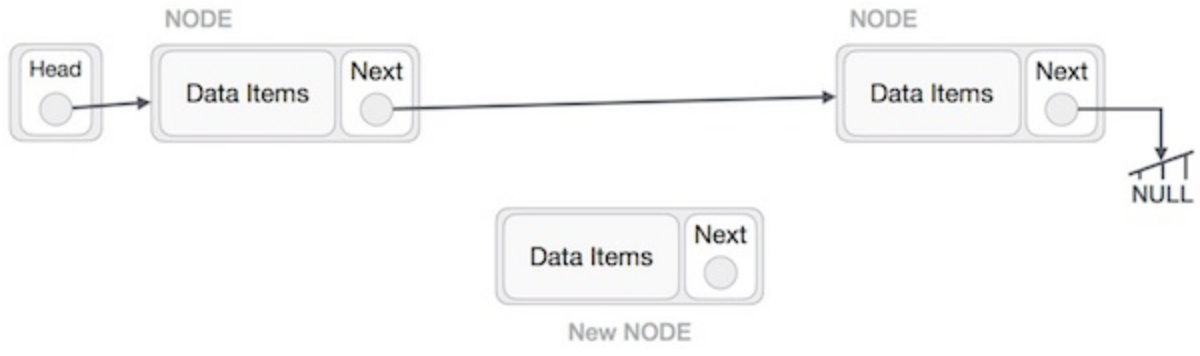
\includegraphics[scale=0.25]{figures/CM2/list-diag-1.png}
        \label{fig:my_label}
    \end{figure}
\end{frame}
\begin{frame}{L'insertion}
    L'ajout d'un nouveau nœud dans une liste chaînée est une activité à plusieurs étapes. Nous allons l'apprendre ici à l'aide de diagrammes. Tout d'abord, créez un nœud en utilisant la même structure et trouvez l'emplacement où il doit être inséré.
    
    \begin{figure}
        \centering
        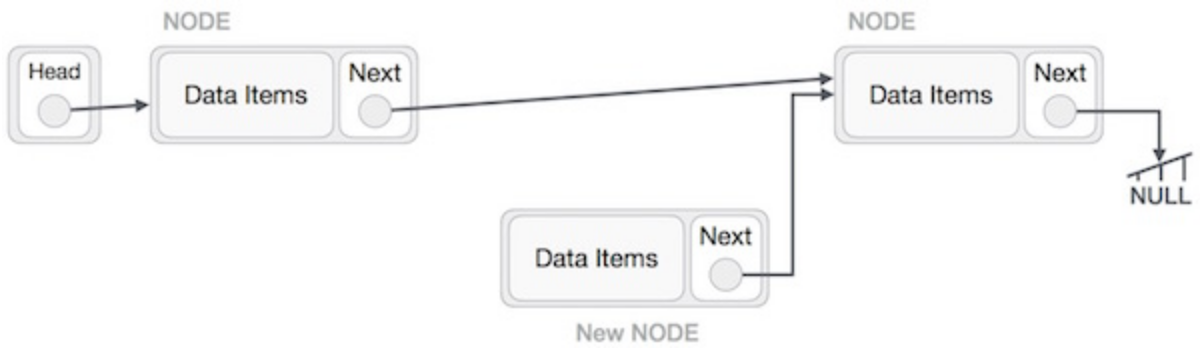
\includegraphics[scale=0.25]{figures/CM2/list-diag-2.png}
        \label{fig:my_label}
    \end{figure}
\end{frame}
\begin{frame}{L'insertion}
    L'ajout d'un nouveau nœud dans une liste chaînée est une activité à plusieurs étapes. Nous allons l'apprendre ici à l'aide de diagrammes. Tout d'abord, créez un nœud en utilisant la même structure et trouvez l'emplacement où il doit être inséré.
    
    \begin{figure}
        \centering
        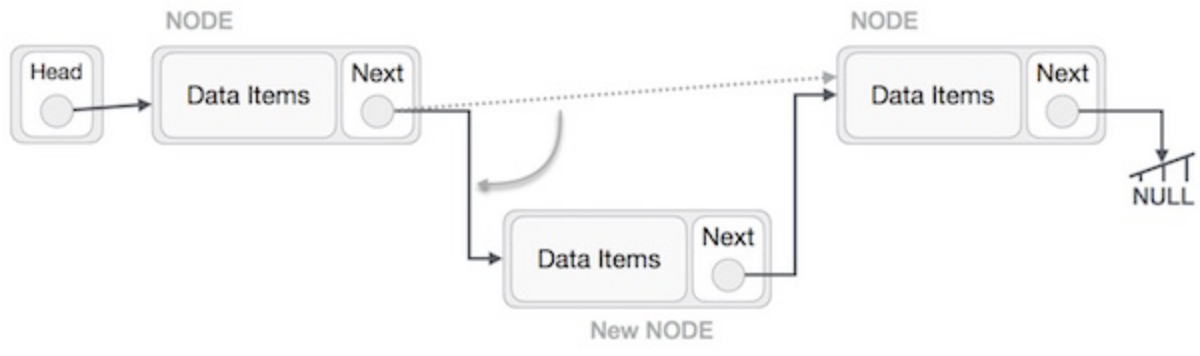
\includegraphics[scale=0.25]{figures/CM2/list-diag-3.png}
        \label{fig:my_label}
    \end{figure}
\end{frame}
\begin{frame}{L'insertion}
    L'ajout d'un nouveau nœud dans une liste chaînée est une activité à plusieurs étapes. Nous allons l'apprendre ici à l'aide de diagrammes. Tout d'abord, créez un nœud en utilisant la même structure et trouvez l'emplacement où il doit être inséré.
    
    \begin{figure}
        \centering
        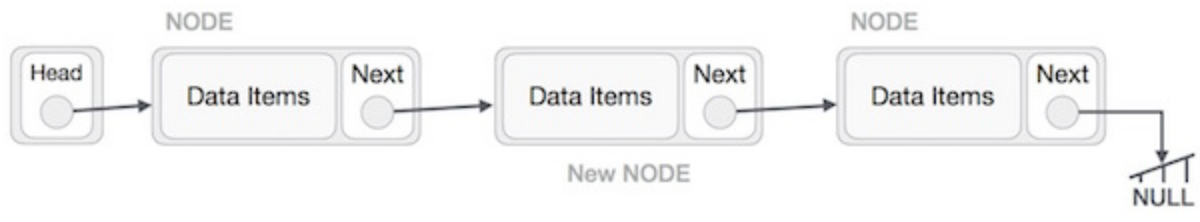
\includegraphics[scale=0.25]{figures/CM2/list-diag-4.png}
        \label{fig:my_label}
    \end{figure}
\end{frame}


\begin{frame}{La suppression d'un élément}
La suppression est également un processus en plusieurs étapes. Nous allons l'apprendre à l'aide d'une représentation graphique. Tout d'abord, il faut localiser le nœud cible à supprimer.
        \begin{figure}
        \centering
        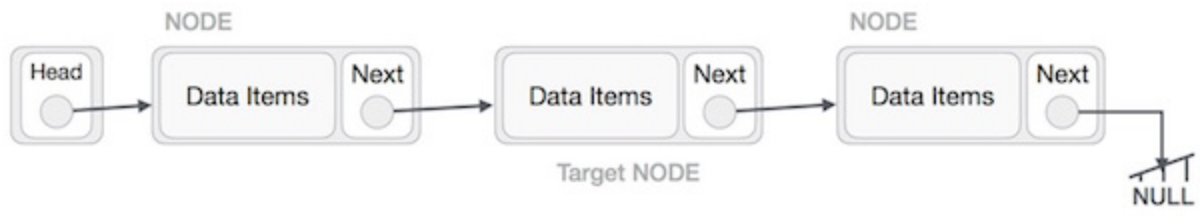
\includegraphics[scale=0.25]{figures/CM2/list-del-1.png}
        \label{fig:my_label}
    \end{figure}
    
\end{frame}

\begin{frame}{La suppression d'un élément}
Le nœud gauche (précédent) du nœud cible doit maintenant pointer vers le nœud suivant du nœud cible.
        \begin{figure}
        \centering
        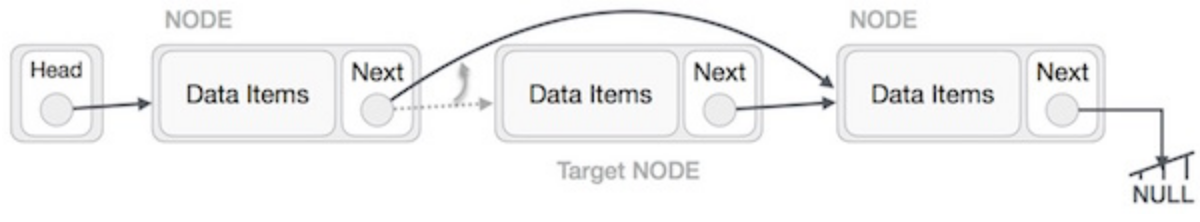
\includegraphics[scale=0.25]{figures/CM2/list-del-2.png}
        \label{fig:my_label}
    \end{figure}
    
\end{frame}

\begin{frame}{La suppression d'un élément}
Cela supprimera le lien qui pointait vers le nœud cible. Maintenant, nous allons supprimer ce vers quoi le noeud cible pointe.
        \begin{figure}
        \centering
        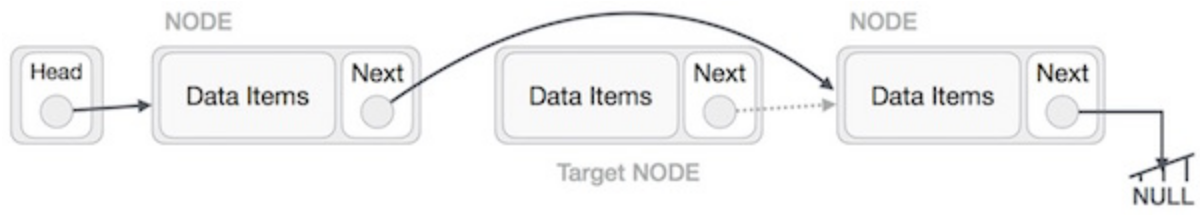
\includegraphics[scale=0.25]{figures/CM2/list-del-3.png}
        \label{fig:my_label}
    \end{figure}
    
\end{frame}

\begin{frame}{La suppression d'un élément}
 Nous pouvons le garder en mémoire, sinon nous pouvons simplement désallouer la mémoire et effacer complètement le nœud cible.
        \begin{figure}
        \centering
        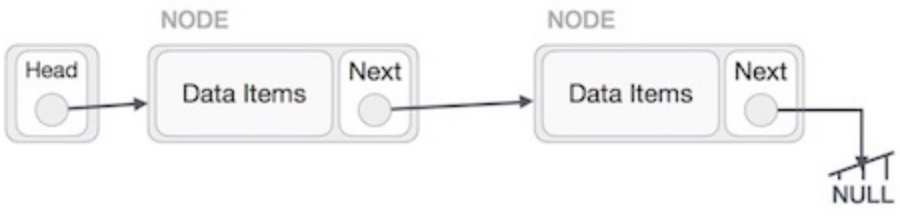
\includegraphics[scale=0.25]{figures/CM2/list-del-4.png}
        \label{fig:my_label}
    \end{figure}
    
\end{frame}

\section{Les files}

\begin{frame}{Les files}
    \begin{exampleblock}{Définition}
    La \defin{file} est une structure de données abstraite, un peu similaire aux piles. Contrairement aux piles, une file d'attente est ouverte à ses deux extrémités.\\
    
    Une extrémité est toujours utilisée pour insérer des données (\textit{enqueue}) et l'autre est utilisée pour retirer des données (\textit{dequeue}).\\
    
    La file d'attente suit la méthodologie "\textit{First-In-First-Out}", c'est-à-dire que l'élément de données stocké en premier sera accédé en premier.
    \end{exampleblock}
    
    \begin{figure}
        \centering
        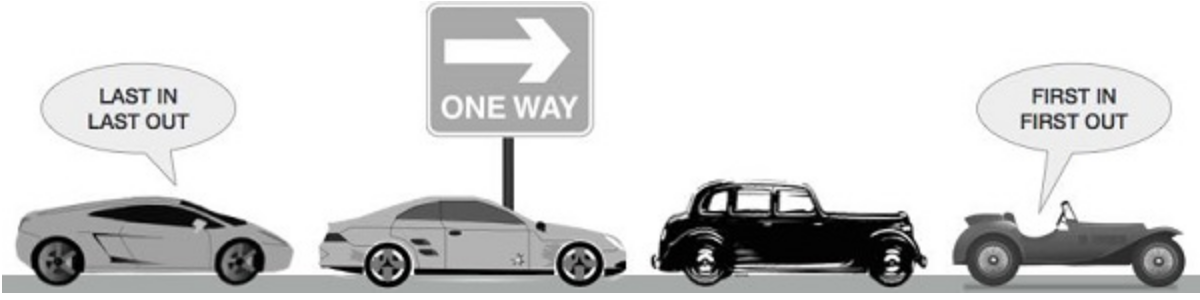
\includegraphics[scale=0.2]{figures/CM2/file-voiture.png}
        \label{fig:my_label}
    \end{figure}
\end{frame}

\begin{frame}{Opérations de base}
    Les opérations sur les files d'attente peuvent consister à initialiser ou à définir la file d'attente, à l'utiliser, puis à l'effacer complètement de la mémoire. Nous allons essayer ici de comprendre les opérations de base associées aux files d'attente :
    
    \begin{itemize}
        \item \alert{\textbf{enqueue()}} : ajoute (stocke) un élément à la file d'attente;
        \item \alert{\textbf{dequeue()}} : retirer (accéder) un élément de la file d'attente;
    \end{itemize}
Quelques fonctions supplémentaires sont nécessaires pour rendre l'opération de file d'attente mentionnée ci-dessus efficace.

\begin{itemize}
    \item \alert{\textbf{peek()}} - Obtient l'élément en tête de la file d'attente sans le retirer;
    \item \alert{\textbf{isfull()}} - Vérifie si la file d'attente est pleine;
    \item \alert{\textbf{isempty()}} - Vérifie si la file d'attente est vide.
\end{itemize}
\end{frame}

\begin{frame}{Ajout d'un élément dans une file}
    Les files d'attente maintiennent deux pointeurs de données, avant et arrière. Par conséquent, leurs opérations sont plus difficiles à mettre en œuvre que celles des piles.

Les étapes suivantes doivent être suivies pour mettre en file d'attente (insérer) des données dans une file d'attente.

\only<1>{
\begin{enumerate}
    \item  Étape 1 - Vérifier si la file d'attente est pleine.
    \item  Étape 2 - Si la file est pleine, produire une erreur de débordement et sortir.
    \item  Étape 3 - Si la file d'attente n'est pas pleine, incrémentez le pointeur arrière pour indiquer le prochain espace vide.
    \item Étape 4 - Ajout d'un élément de données à l'emplacement de la file d'attente, où le pointeur arrière pointe.
\end{enumerate}
 }
 
 \only<2>{
 
 \begin{figure}
     \centering
     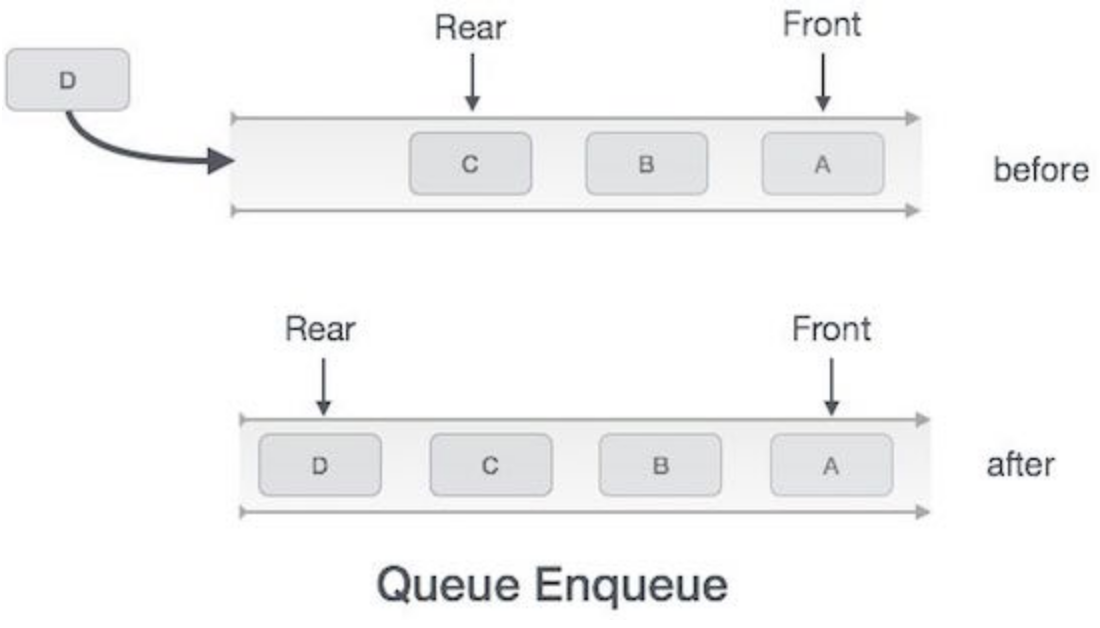
\includegraphics[scale=0.2]{figures/CM2/file-ins.png}
     \label{fig:my_label}
 \end{figure}
 }
\end{frame}


\begin{frame}{Retirer/accéder à un élément}
    L'accès aux données de la file d'attente est un processus composé de deux tâches - accéder aux données où le front est pointé et retirer les données après l'accès. 
    Les étapes suivantes sont suivies pour effectuer l'opération de dequeue

\only<1>{
\begin{enumerate}
    \item Étape 1 - Vérifier si la file d'attente est vide.
    \item Étape 2 - Si la file d'attente est vide, produire une erreur de dépassement de capacité et sortir.
    \item Étape 3 - Si la file d'attente n'est pas vide, accéder aux données sur lesquelles le pointeur frontal pointe.
    \item Étape 4 - Incrémente le pointeur frontal pour qu'il pointe sur le prochain élément de données disponible.
\end{enumerate}
}

\only<2>{
\begin{figure}
    \centering
    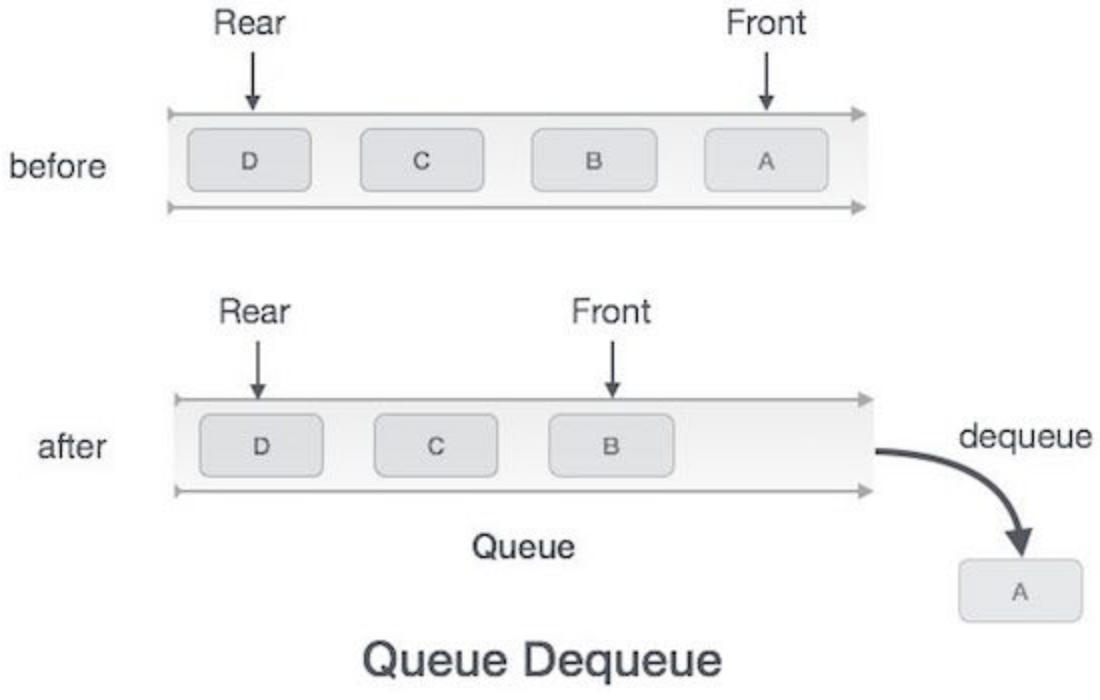
\includegraphics[scale=0.2]{figures/CM2/file-del.png}
    \label{fig:my_label}
\end{figure}
}

\end{frame}


\section{Les arbres}

\begin{frame}{Les arbres binaires}
    \begin{exampleblock}{Définition}
    \defin{L'arbre binaire} est une structure de données spéciale utilisée à des fins de stockage de données. Un arbre binaire a une condition spéciale : chaque nœud peut avoir un maximum de deux enfants.
    \end{exampleblock}
    \begin{figure}
    \centering
    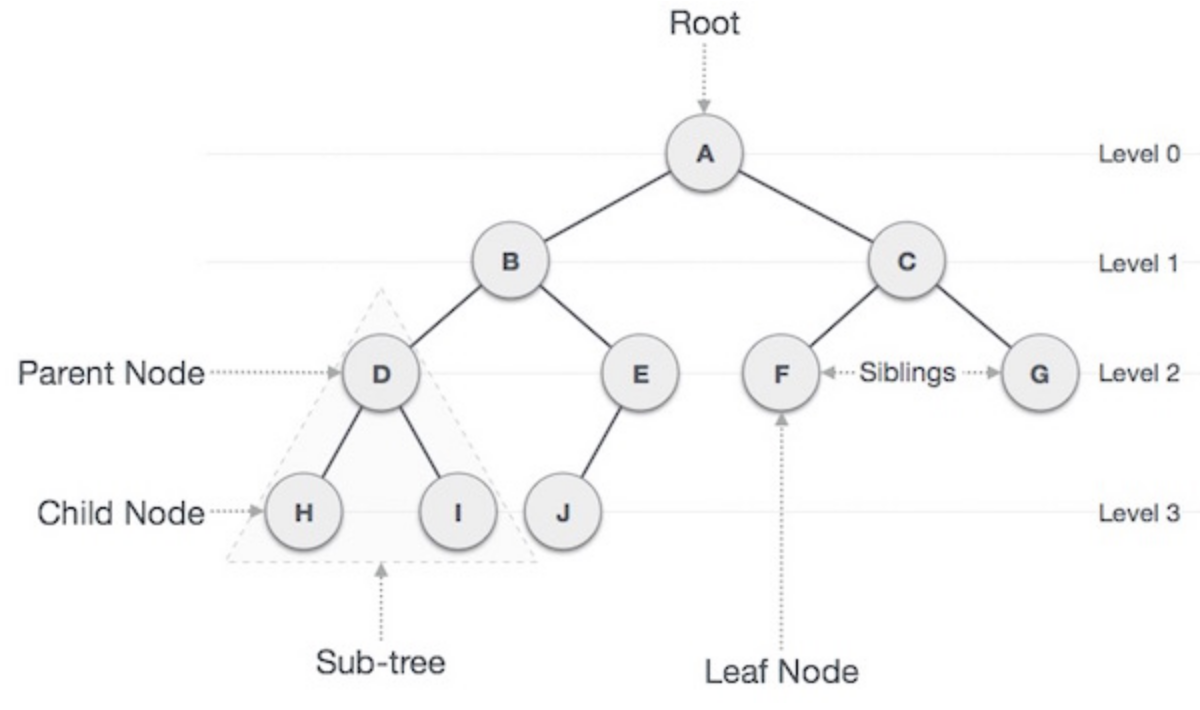
\includegraphics[scale=0.2]{figures/CM2/ABR-1.png}
    \label{fig:my_label}
\end{figure}
    
\end{frame}

\begin{frame}{Vocabulaire sur les arbres}
    \begin{exampleblock}{Chemin}
    Le \defin{chemin} fait référence à la séquence de nœuds le long des bords d'un arbre.
    \end{exampleblock}
    
    \begin{figure}
    \centering
    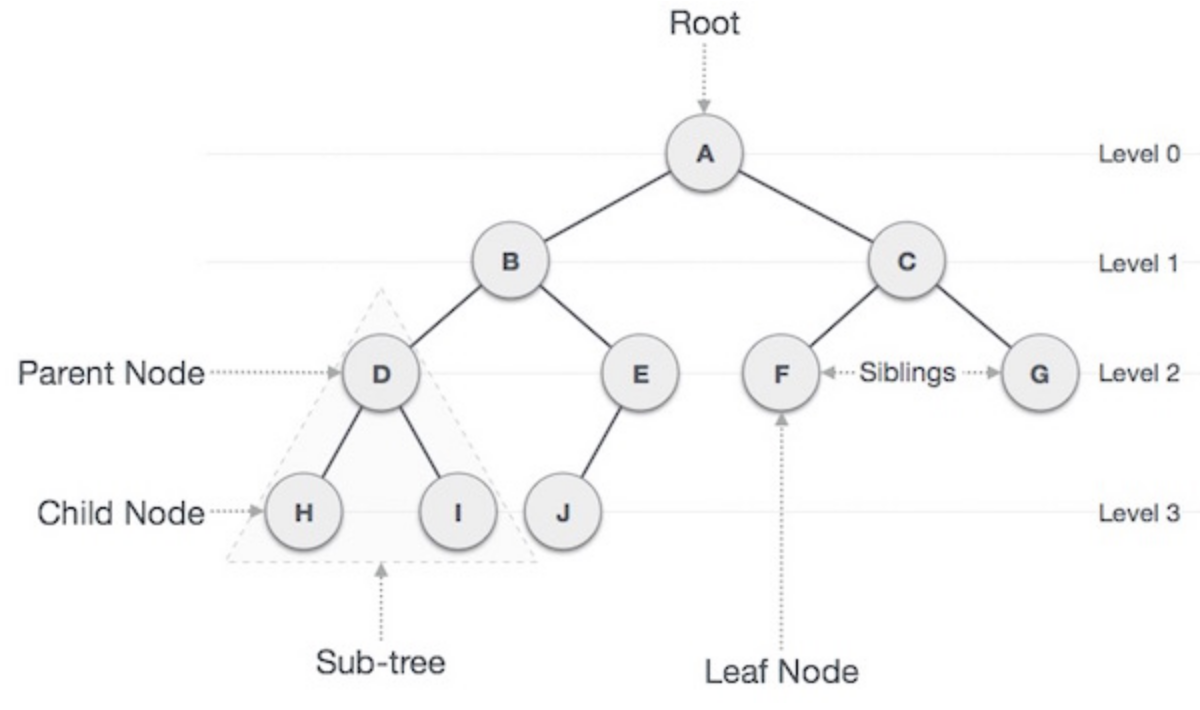
\includegraphics[scale=0.2]{figures/CM2/ABR-1.png}
    \label{fig:my_label}
\end{figure}
\end{frame}

\begin{frame}{Vocabulaire sur les arbres}
    \begin{exampleblock}{Racine}
     Le nœud situé au sommet de l'arbre est appelé \defin{racine}. Il n'y a qu'une seule racine par arbre et un seul chemin du nœud racine vers n'importe quel nœud.
    \end{exampleblock}
    
    \begin{figure}
    \centering
    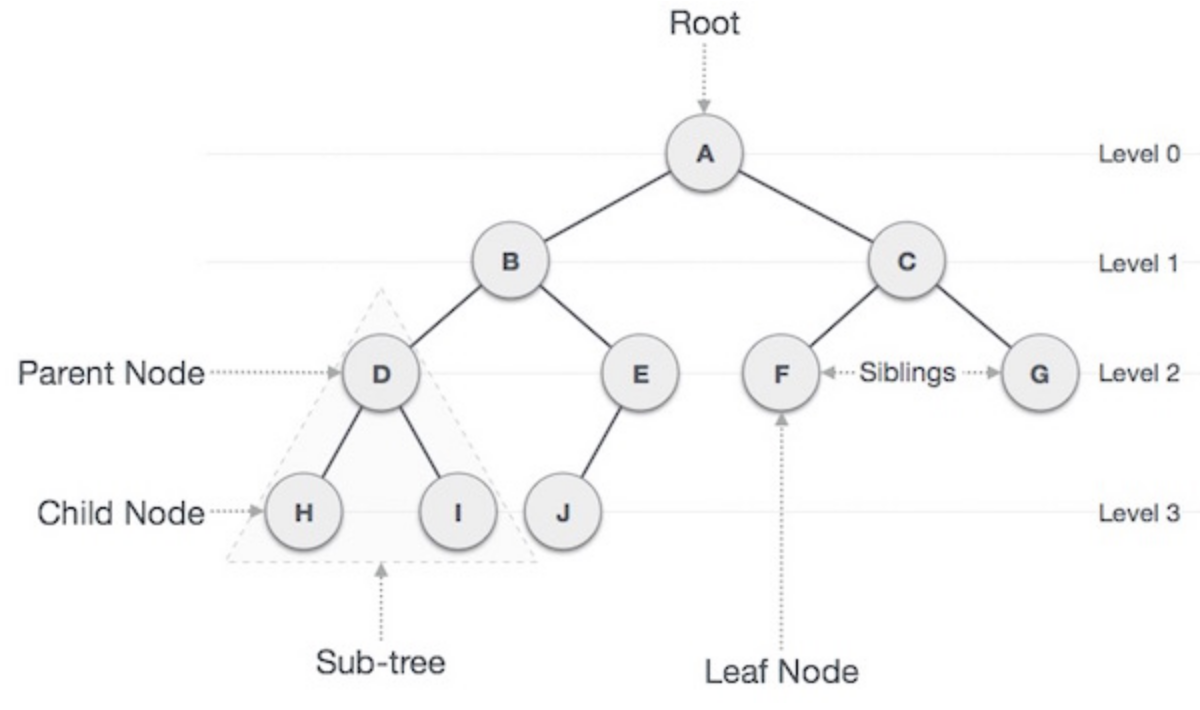
\includegraphics[scale=0.2]{figures/CM2/ABR-1.png}
    \label{fig:my_label}
\end{figure}
\end{frame}

\begin{frame}{Vocabulaire sur les arbres}
    \begin{exampleblock}{Parent}
    Tout nœud, à l'exception du nœud racine, possédant une arête ascendante vers un nœud appelé \defin{parent}.
    \end{exampleblock}
    
    \begin{figure}
    \centering
    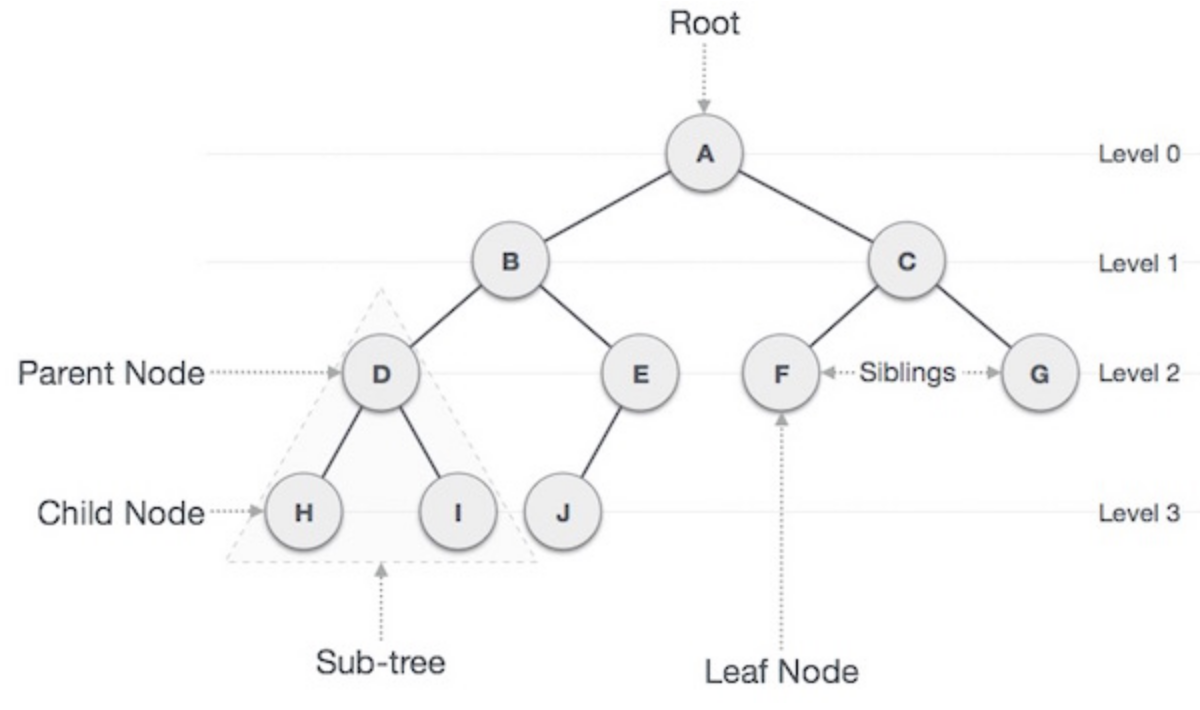
\includegraphics[scale=0.2]{figures/CM2/ABR-1.png}
    \label{fig:my_label}
\end{figure}
\end{frame}

\begin{frame}{Vocabulaire sur les arbres}
    \begin{exampleblock}{Enfant}
    Le nœud situé sous un nœud donné et relié par son bord descendant est appelé nœud \defin{enfant}.
    \end{exampleblock}
    
    \begin{figure}
    \centering
    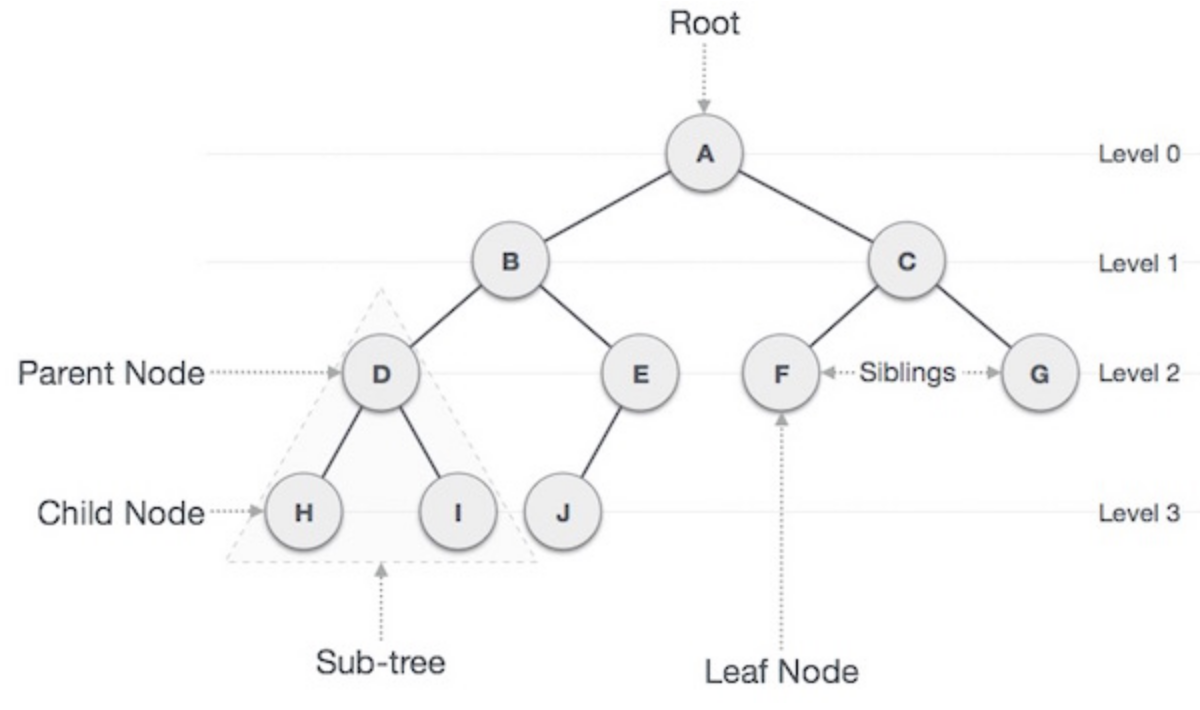
\includegraphics[scale=0.2]{figures/CM2/ABR-1.png}
    \label{fig:my_label}
\end{figure}
\end{frame}

\begin{frame}{Vocabulaire sur les arbres}
    \begin{exampleblock}{Feuille}
    Le nœud qui n'a pas de nœud enfant est appelé nœud \defin{feuille}.
    \end{exampleblock}
    
    \begin{figure}
    \centering
    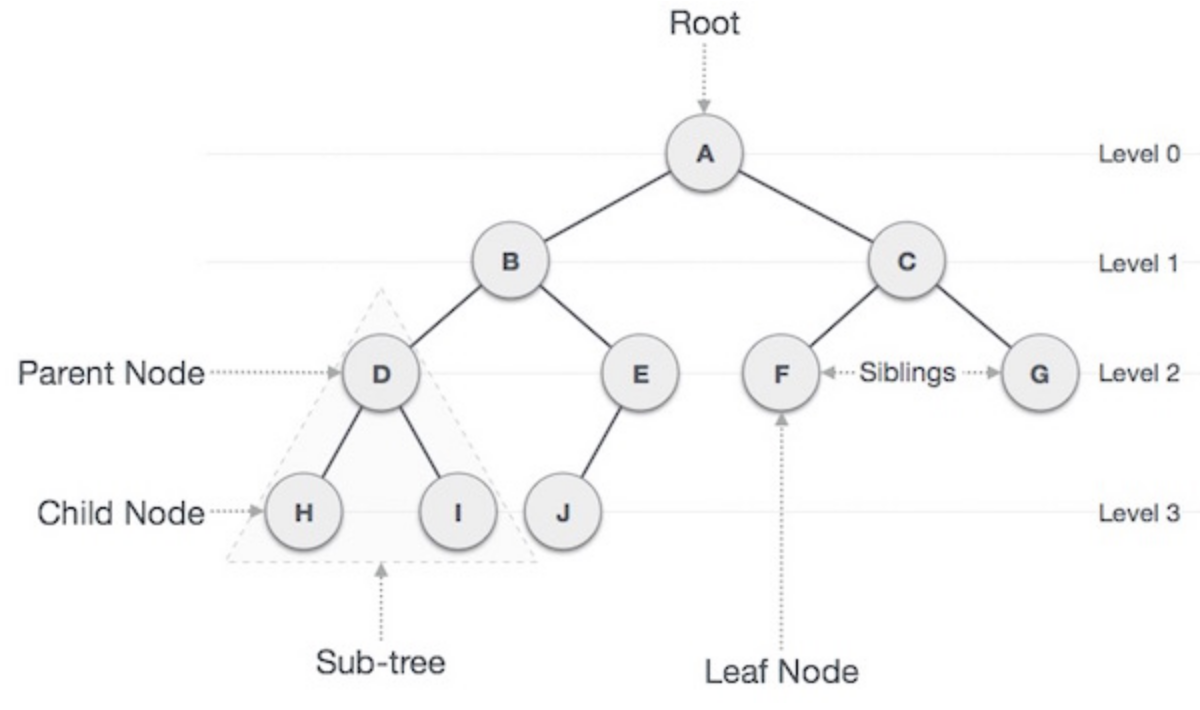
\includegraphics[scale=0.2]{figures/CM2/ABR-1.png}
    \label{fig:my_label}
\end{figure}
\end{frame}

\begin{frame}{Vocabulaire sur les arbres}
        \begin{exampleblock}{sous-arbre}
   Le \defin{sous-arbre} représente les descendants d'un nœud.
    \end{exampleblock}
    
    \begin{figure}
    \centering
    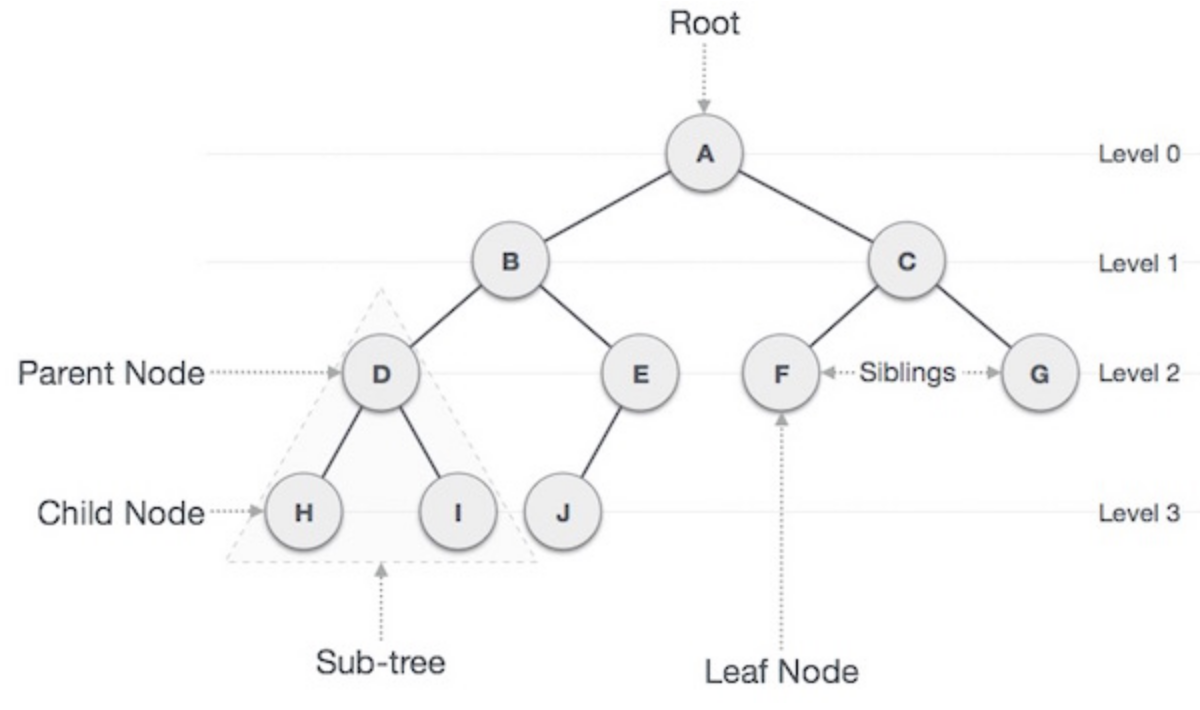
\includegraphics[scale=0.2]{figures/CM2/ABR-1.png}
    \label{fig:my_label}
\end{figure}
\end{frame}

\begin{frame}{Vocabulaire sur les arbres}
        \begin{exampleblock}{Visiter}
    \defin{Visiter} signifie vérifier la valeur d'un nœud lorsque le contrôle est sur le nœud.
    \end{exampleblock}
    
    \begin{figure}
    \centering
    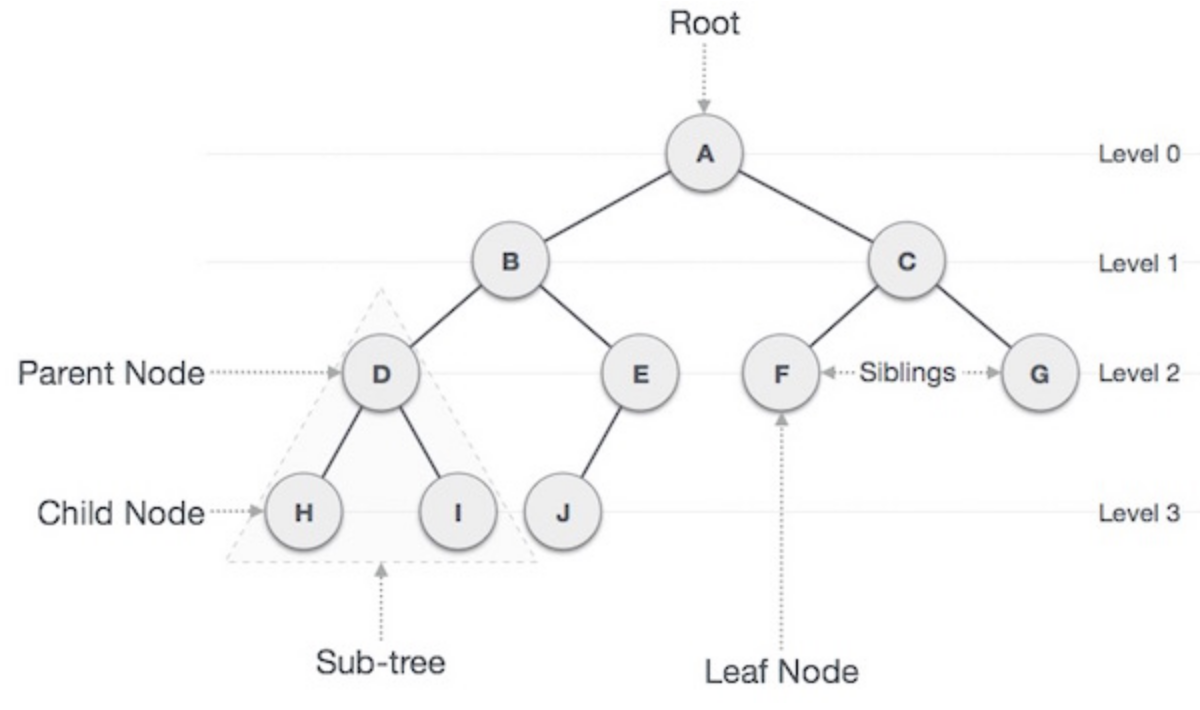
\includegraphics[scale=0.2]{figures/CM2/ABR-1.png}
    \label{fig:my_label}
\end{figure}
\end{frame}

\begin{frame}{Vocabulaire sur les arbres}
        \begin{exampleblock}{Parcours}
    Le \defin{parcours} consiste à passer par les nœuds dans un ordre spécifique.
    \end{exampleblock}
    
    \begin{figure}
    \centering
    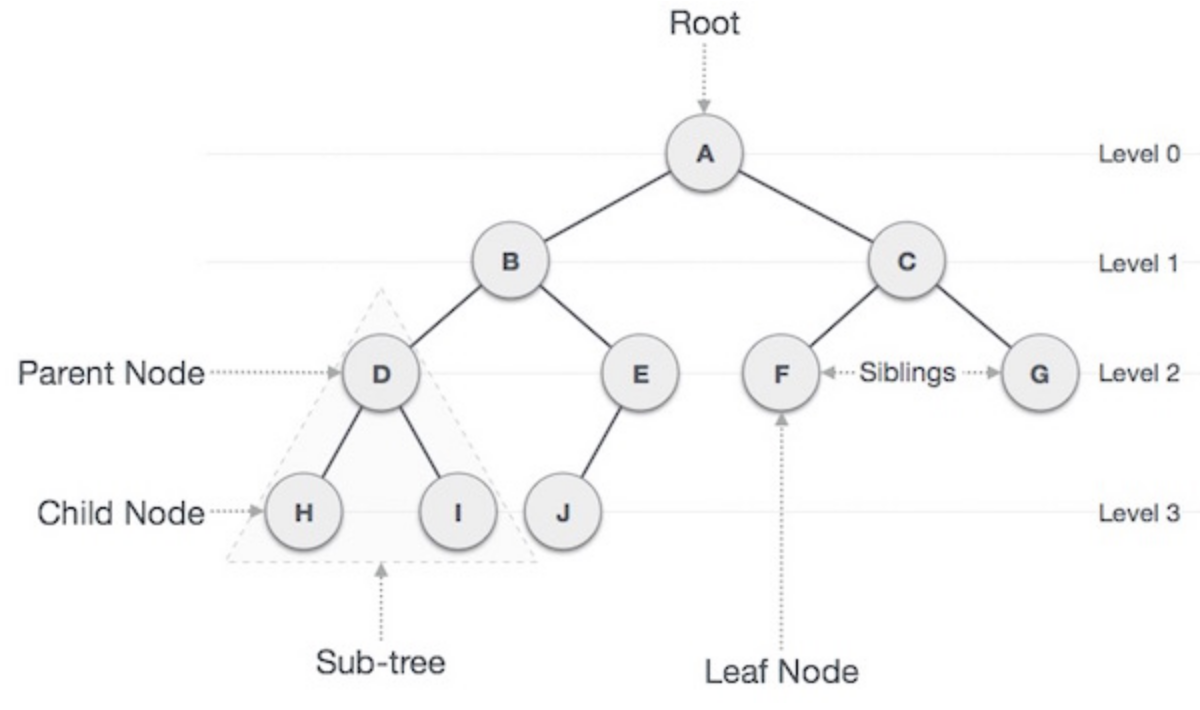
\includegraphics[scale=0.2]{figures/CM2/ABR-1.png}
    \label{fig:my_label}
\end{figure}
\end{frame}

\begin{frame}{Vocabulaire sur les arbres}
        \begin{exampleblock}{Niveaux}
    Le \defin{niveau} d'un nœud représente la génération d'un nœud. Si le nœud racine se trouve au niveau 0, alors son nœud enfant suivant se trouve au niveau 1, son petit-enfant se trouve au niveau 2, et ainsi de suite.
    \end{exampleblock}
    
    \begin{figure}
    \centering
    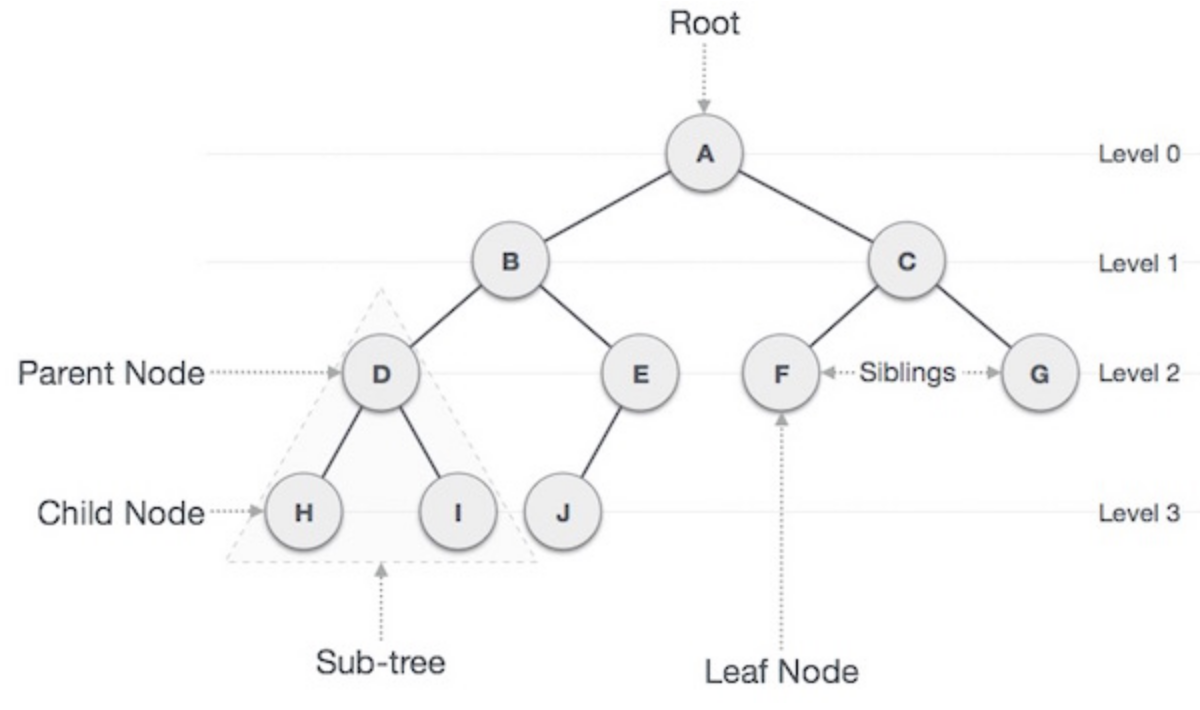
\includegraphics[scale=0.2]{figures/CM2/ABR-1.png}
    \label{fig:my_label}
\end{figure}
\end{frame}

\begin{frame}{Vocabulaire sur les arbres}
        \begin{exampleblock}{Clés}
    La \defin{clé} représente une valeur d'un nœud sur la base de laquelle une opération de recherche doit être effectuée pour un nœud.
    \end{exampleblock}
    
    \begin{figure}
    \centering
    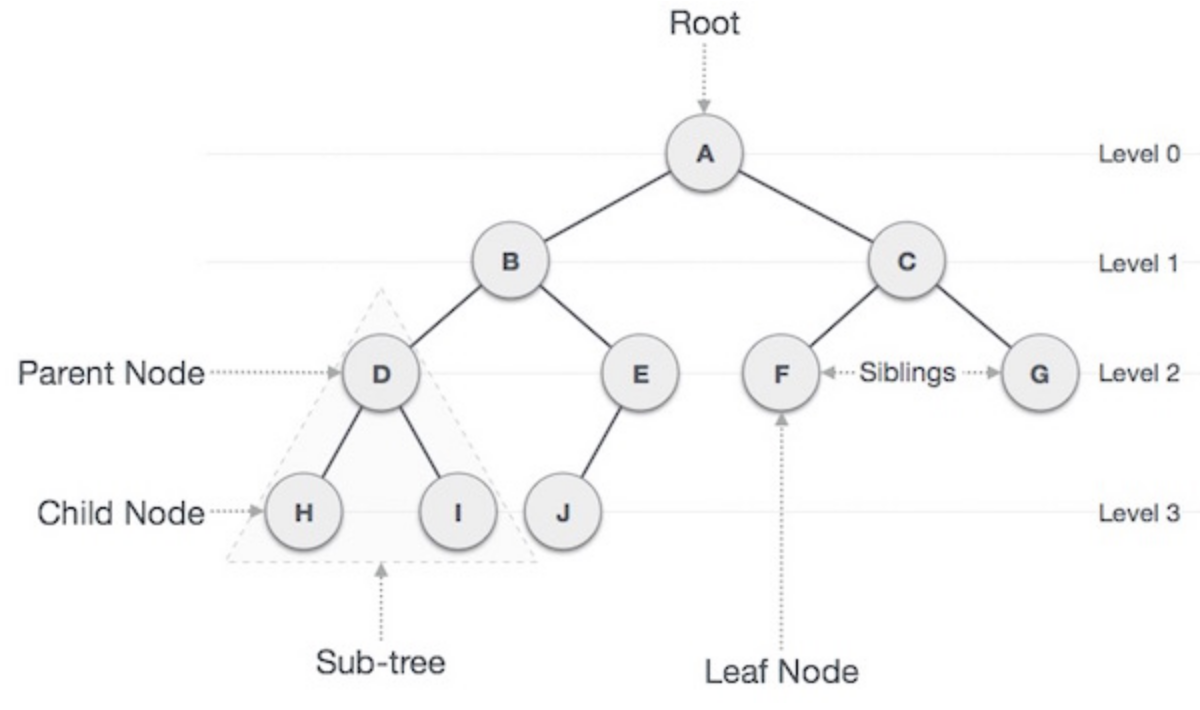
\includegraphics[scale=0.2]{figures/CM2/ABR-1.png}
    \label{fig:my_label}
\end{figure}
\end{frame}

\begin{frame}{Représentation d'un arbre binaire de recherche}
    \alert{L'arbre de binaire de recherche} (ou ABR)  présente un comportement particulier. L'enfant gauche d'un nœud doit avoir une valeur inférieure à celle de son parent et l'enfant droit du nœud doit avoir une valeur supérieure à celle de son parent.
    
    \begin{figure}
    \centering
    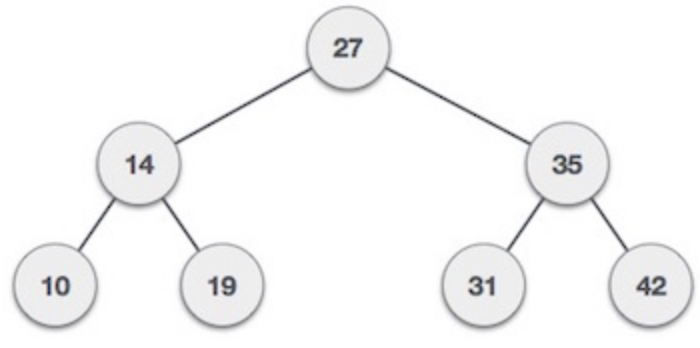
\includegraphics[scale=0.3]{figures/CM2/ABR-2.png}
    \label{fig:my_label}
\end{figure}
    
\end{frame}

\begin{frame}{Opérations de base}
    Les opérations de base qui peuvent être effectuées sur une structure de données d'arbre de recherche binaire sont les suivantes :
    
    \begin{itemize}
        \item \textbf{\alert{Insertion}} : Insère un élément dans un arbre/créer un arbre;
        \item \textbf{\alert{Recherche}} :  Recherche d'un élément dans un arbre;
        \item \textbf{\alert{Parcours préfixe}}  : Parcours un arbre de manière pré-ordonnée;
        \item \textbf{\alert{Parcours infixe}}  : Parcours un arbre dans l'ordre;
        \item \textbf{\alert{Parcours postfixe}}  : Parcours un arbre de manière post-ordonnée;

    \end{itemize}
\end{frame}


\begin{frame}{L'insertion d'un élément}
    La toute première \alert{insertion} crée l'arbre. Par la suite, chaque fois qu'un élément doit être inséré, il faut d'abord localiser son emplacement approprié. Commencez la recherche à partir du noeud racine, puis si les données sont inférieures à la valeur clé, recherchez l'emplacement vide dans le sous-arbre de gauche et insérez les données. Sinon, recherchez l'emplacement vide dans le sous-arbre de droite et insérez les données.
    
    \only<2>{\begin{center}
        \alert{Quel serait l'algorithme ? A vous de jouer !}
    \end{center}}
\end{frame}

\begin{frame}{La recherche d'un élément}
    Lorsqu'un élément doit être \alert{recherché}, la recherche commence à partir du nœud racine, puis si les données sont inférieures à la valeur de la clé, l'élément est recherché dans le sous-arbre de gauche. Sinon, recherchez l'élément dans le sous-arbre de droite. Suivez le même algorithme pour chaque nœud.
    
        \only<2>{\begin{center}
        \alert{Quel serait l'algorithme ? A vous de jouer !}
    \end{center}}
\end{frame}

\begin{frame}{Les parcours}
        \begin{exampleblock}{Parcours}
    Le \defin{parcours} consiste à passer par les nœuds dans un ordre spécifique.
    \end{exampleblock}
    
    Étant donné que tous les nœuds sont reliés par des arêtes, nous commençons toujours par le nœud racine. Il y a trois façons de parcourir un arbre.

\begin{itemize}
    \item Parcours infixe
    \item Parcours préfixe
    \item Parcours suffixe
\end{itemize}

En général, nous parcourons un arbre pour rechercher ou localiser un élément ou une clé donnée dans l'arbre ou pour imprimer toutes les valeurs qu'il contient.
\end{frame}

\begin{frame}{Parcours infixe}
    Dans ce \alert{parcours}, le sous-arbre de gauche est visité en premier, puis la racine et enfin le sous-arbre de droite. Il faut toujours se rappeler que chaque nœud peut représenter un sous-arbre lui-même.

Si un arbre binaire est parcouru dans l'ordre, la sortie produira des valeurs de clés triées dans un ordre croissant.

\begin{figure}
    \centering
    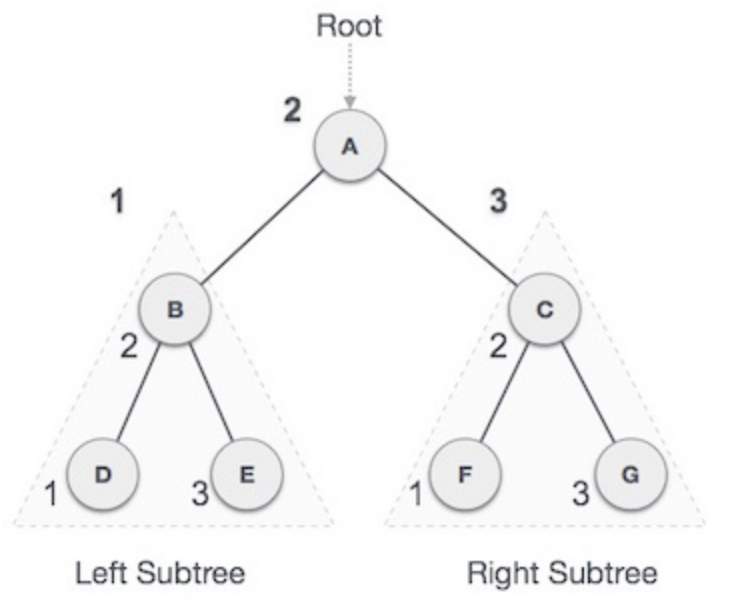
\includegraphics[scale=0.2]{figures/CM2/ABR-infix.png}
    \label{fig:my_label}
\end{figure}
\end{frame}

\begin{frame}{Parcours infixe}

\begin{figure}
    \centering
    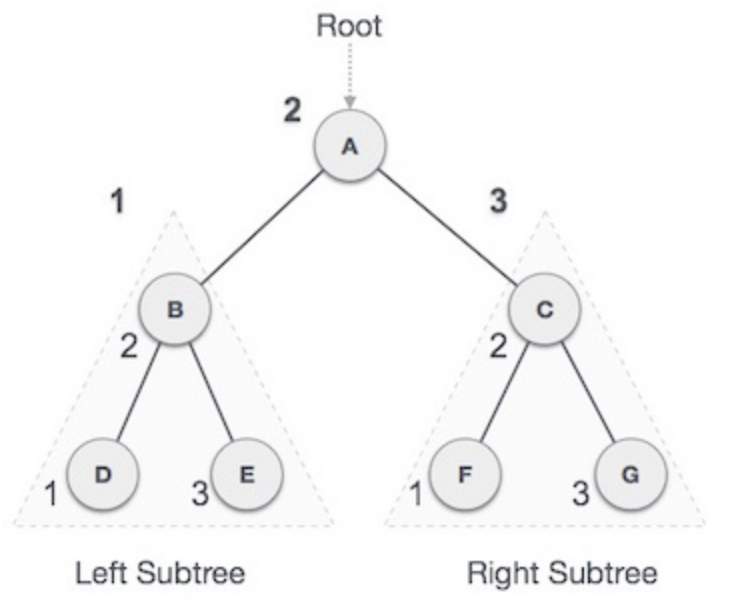
\includegraphics[scale=0.25]{figures/CM2/ABR-infix.png}
    \label{fig:my_label}
\end{figure}

\alert{\begin{center}
    Qu'obtiendrait-on dans cet exemple ?\\
    \only<2>{$D \rightarrow B \rightarrow E\rightarrow A\rightarrow F\rightarrow C\rightarrow G$}
\end{center}}
\end{frame}

\begin{frame}{Ébauche d'algorithme}
    \begin{alertblock}{Algorithme}
    Tant que tout les les noeuds ne sont pas parcouru :
    \begin{enumerate}
        \item Étape 1 - Parcourir récursivement le sous-arbre de gauche.
        \item Étape 2 - Visite du noeud racine.
        \item Étape 3 - Parcourez récursivement le sous-arbre de droite.
    \end{enumerate}
    \end{alertblock}
\end{frame}

\begin{frame}{Le parcours préfixe}
    Dans ce \alert{parcours}, le nœud racine est visité en dernier, d'où son nom. Nous parcourons d'abord le sous-arbre de gauche, puis le sous-arbre de droite et enfin le nœud racine.
    
    \begin{figure}
    \centering
    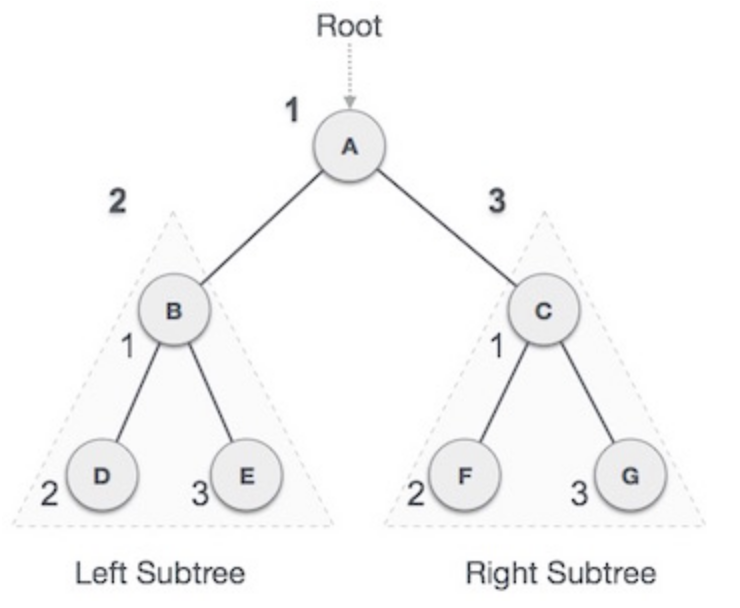
\includegraphics[scale=0.2]{figures/CM2/ABR-pref.png}
    \label{fig:my_label}
\end{figure}
\end{frame}

\begin{frame}{Le parcours préfixe}

\begin{figure}
    \centering
    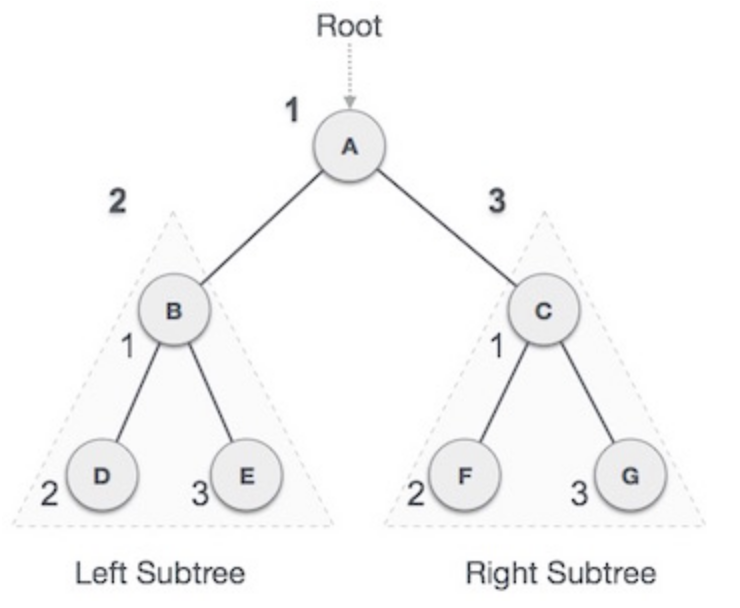
\includegraphics[scale=0.25]{figures/CM2/ABR-pref.png}
    \label{fig:my_label}
\end{figure}

\alert{\begin{center}
    Qu'obtiendrait-on dans cet exemple ?\\
    \only<2>{$D \rightarrow E \rightarrow B\rightarrow F\rightarrow G\rightarrow C\rightarrow A$}
\end{center}}
\end{frame}


\begin{frame}{Ébauche d'algorithme}
    \begin{alertblock}{Algorithme}
    Tant que tout les les noeuds ne sont pas parcouru :
    \begin{enumerate}
        \item Étape 1 - Parcourir récursivement le sous-arbre de gauche.
        \item Étape 2 - Parcourez récursivement le sous-arbre de droite.
        \item Étape 3 - Visite du noeud racine.
    \end{enumerate}
    \end{alertblock}
\end{frame}

\end{document}